

The whole project encompasses different libraries, prototypes and applications.
This chapter describes the design of each part of the product in detail,
and documents the various approaches taken into consideration.

\section{System overview}

The system consists of:
\begin{description}
	\item[Libraries:] Social library, Communication Library
	\item[Applications:] T-Shirt application, other applications
	\item[Prototypes:] T-Shirt prototype, other prototypes
\end{description}

The figure \ref{fig:design-toplevel} illustrates the overall system architecture.

\begin{figure}[h!]
\centering 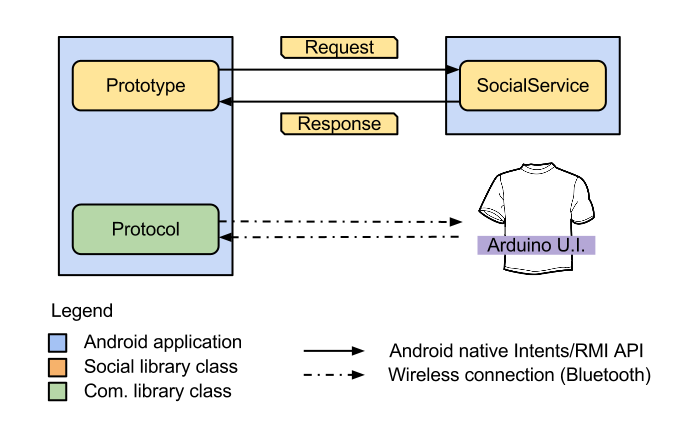
\includegraphics[scale=0.35]{img/design-toplevel.png}
\caption{Overall system architecture}
\label{fig:design-toplevel}
\end{figure}

\newpage
\section{System design}
As the requirements for the product were not set early on by the customer, a lot of effort
was put into producing working prototypes to show during the meetings in order to receive
as much feedback as possible and identify the ideas the customer had in mind.
These would provide what was needed to proceed with system design.
At some point thou, after roughly one month, we understood that we were going in the wrong direction,
and that our design wouldn't satisfy the requirements for the use cases the customer mentioned and the
design of some parts of the system had to be revised. It involved especially the Social library and both
the Facebook and T-Shirt applications.

\subsection{First design}
Our first system design was based on the scenario where the user would download the t-shirt
and the social applications, browse for some content from within the social application
and actively send it to the t-shirt application pressing a 'share' button.
This scenario is illustrated in figure \ref{fig:design-usecase1}.

\begin{figure}[h!]
\centering 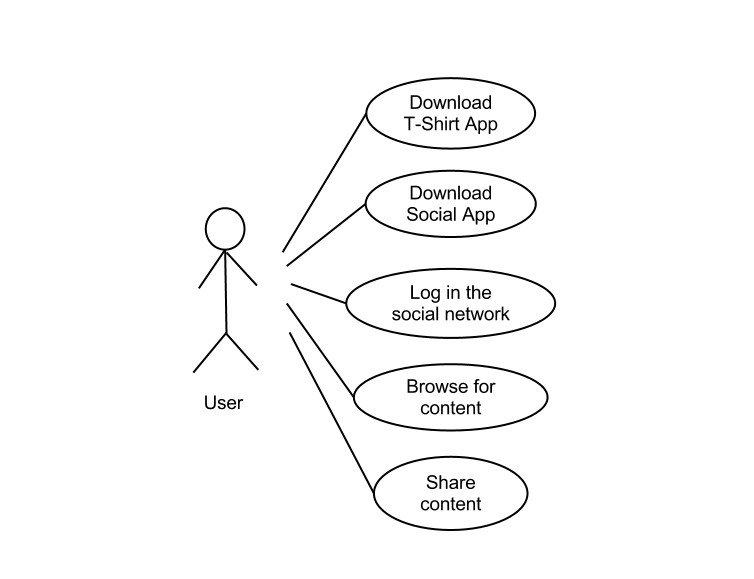
\includegraphics[scale=0.35]{img/design-usecase1}
\caption{Use case for the product (first design)}
\label{fig:design-usecase1}
\end{figure}

Please note that in this scenario the user is required to actively send data from
the social application (which acts as a Facebook client) to the T-Shirt application,
which is merely capable of receiving. Also, both are implemented as Android applications.

\newpage

The figure \ref{fig:design-resp} represents the communication between the applications.

\begin{figure}[h!]
\centering 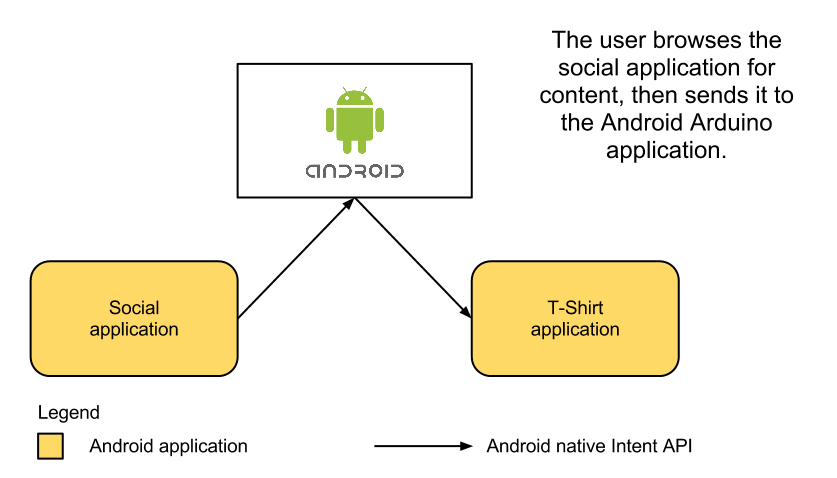
\includegraphics[scale=0.35]{img/design-resp.png}
\caption{Communication diagram (first design)}
\label{fig:design-resp}
\end{figure}


\subsection{Second design}
It turned out that the user was not supposed to browse for social content and send it actively
to the T-Shirt application. Instead, after downloading the software, he would just setup a set of rules
specifying the behavior of the T-Shirt. This scenario is illustrated in figure \ref{fig:design-usecase2}

\begin{figure}[h!]
\centering 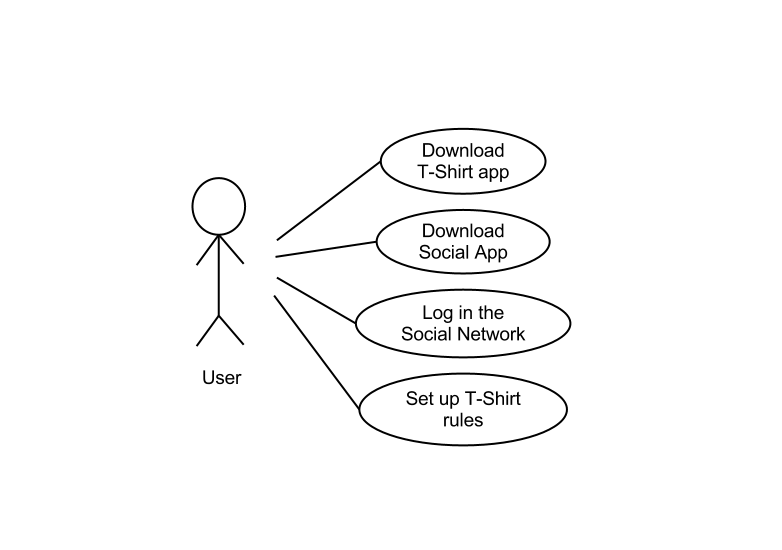
\includegraphics[scale=0.35]{img/design-usecase2}
\caption{Use case for the product (second design)}
\label{fig:design-usecase2}
\end{figure}

This new scenario made clear that that both the Social and the T-Shirt applications needed to
be split into:

\begin{itemize}
\item A user interface, implemented as one or more Android applications, that the user could use to
authenticate within the social network and setup the rules for the T-Shirt.
\item Two Android services that would run in the background, without user interaction,
to fetch data from the social networks and forward it to the Arduino.
\end{itemize}

It also implied that a mechanism to request and exchange social content had to be provided
by the Social library. The figure \ref{fig:design-reqresp} illustrates the communication between
the services and the applications.

\begin{figure}[h!]
\centering 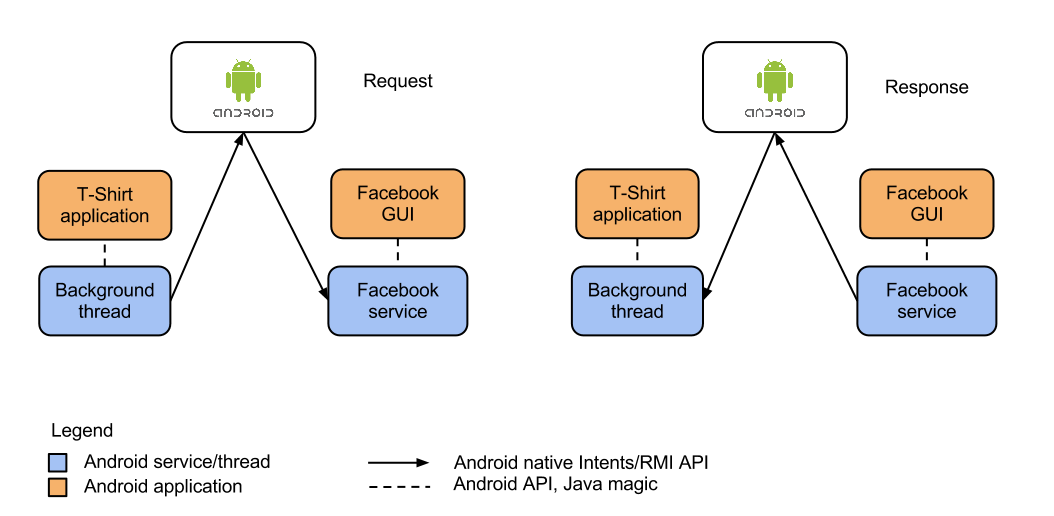
\includegraphics[scale=0.35]{img/design-reqresp.png}
\caption{Communication diagram (second design)}
\label{fig:design-reqresp}
\end{figure}

The T-Shirt service is now 'asking' the Social service for a specific content.
This happens in the background, without user interaction.

\newpage

\subsubsection{Sequence Diagram}
This sequence diagram shows a sample communication between the Social and T-Shirt applications.
The T-Shirt application requests the list of friends from Facebook whose age is the same as 'Anna'.

\begin{figure}[h!]
\centering 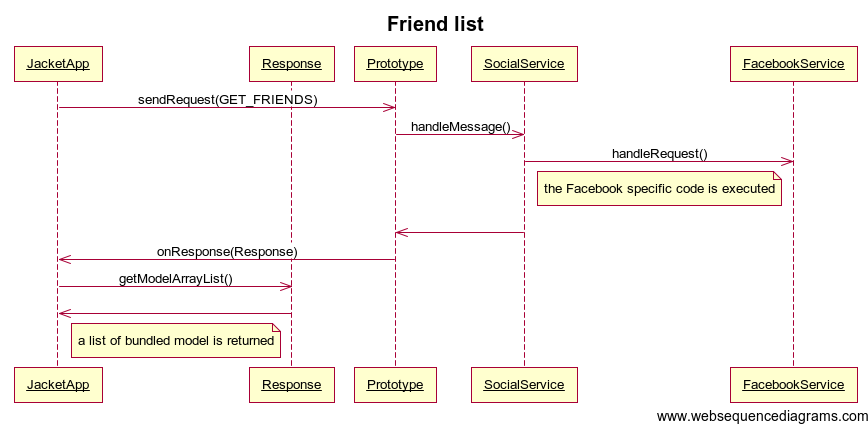
\includegraphics[width=1.0\textwidth]{img/design-sequence.png}
\caption{Sequence diagram}
\label{fig:design-sequence}
\end{figure}

\newpage

\section{Libraries}

\subsection{The Social library}
This library provides abstractions for many common concepts found in different
social networks like Facebook, OpenSocial.. in order to give the developers the possibility
to use these concepts seamlessly between these networks and extend them to possibily support others.
It also defines and implements a sort of 'protocol' to allow Android applications and/or services
to exchange social data. This mechanism is based on Android Intent's API.

\subsubsection{First approach}
Our first design approach consisted in a library that would handle the connection to social networks
such as Facebook, Twitter, LinkedIn and so on, allowing the developers to write full-fledged
social 'multi-network' clients. It would also provide abstractions for many common concepts
found in these networks such as Post, User, Comment and so on.

\subsubsection{Revised approach}
The difference in the new approach is that while the Social library will still provide
abstractions for common concepts found in social networks, it will now focus rather than handling
the connection to the social networks, on estabilishing a communication interface (using Android's Intent mechanism)
between Social applications and the Android-Arduino applications to allow the requesting and forwarding of social data.

This revised approach was made necessary after the first meetings with the customer
as we misunderstood the project scope and went on to solve a very ambitious and unneeded task.
The new design also accomodated very well the overall system design. Some of the code and documentation we produced
for the previous design was re-used, but some could not.

\todo{
	a class diagram maybe?
}

\newpage

\subsection{The Communication library}
This library consists of a Java library and an Arduino firmware. Both implement the ComLib protocol.
The Java library provides a set of classes that allow to easily connect to Arduino devices that run the Communication library
Arduino firmware. The library also implements a mechanism to manage Arduino's firmware, allowing the device to support
different hardware configurations. Wait, Really?

\todo{
	a class diagram maybe?
}

\subsubsection{The ComLib Protocol}
The protocol is a basic set of rules that define how devices can communicate to the Arduino.
The ComLib protocol itself was designed by us, and has seen much changes in terms of which instructions were to be included,
and how the communication was to be executed. With the current design the Arduino cannot initiate the communication,
but is instead a passive device. For all instructions sent by any device to the Arduino, the Arduino sends a response,
either to acknowledge that it is finished executing the corresponding tasks, or the actually return the required
information in the "Content" field. An overview of the current instructions in the protocol can be seen in Table~\ref{tbl:opcodes}.

\begin{table}[h!]
\begin{tabular}{ | c | c | p{1.5cm} | p{1.7cm} | p{6cm} |}
\hline
\textbf{Name} & \textbf{OPCODE} & \textbf{Flag} & \textbf{Content} & \textbf{Description} \\
\hline
Ping & 0x00 & N/A & N/A & Pings the arduino, to check that it's there \\
\hline
Text & 0x01 & N/A & Text to send & Sends text to the arduino, which then displays it depending on the implementation on the ardunio \\
\hline
Sensor & 0x02 & Sensor number & N/A & Requests sensor information from the arduino \\
\hline
Pin pulse & 0x03 & Pin number & N/A & Sends a 500ms pulse on the specified pin \\
\hline
Pin read & 0x04 & Pin number & N/A & Reads the current digital state of the specified pin on the arduino \\
\hline
Pin write & 0x05 & Pin number & Pin value (0~or1) & Writes a digital state of a pin on the arduino \\
\hline
Response & 0xFE & Opcode & Response content & A response to a previous instruction, where the flag is the opcode for which it is the response to \\
\hline
Reset & 0xFF & N/A & N/A & Resets the arduino \\
\hline
\end{tabular}
\caption{Overview of the protocol's instructions}
\label{tbl:opcodes}
\end{table}

\subsubsection{Arduino firmware implementation}
On the Arduino, all code related to our protocol is abstracted into a ComputerSerial library.
This library is a very basic state machine which processes single bytes received (see Figure~\ref{fig:arduino_states}).
The user of this library can register local methods to be called with RPC when the corresponding instruction is called.
The instructions follow strict rules on how they are constructed (see Table~\ref{tbl:instr_struct} for sizes of the different parts).
Each instruction has to start with a "start-byte" which is always 0xFF. The next part is the size, which tells the number of bytes
to come for this instruction (including the size byte itself). The rest is defined from which instruction is sent, but it is important to
remember that the content cannot be empty, and has to at least contain 1 byte. This byte however, is not necessarily read or used.

The following figure illustrates the Arduino automata.

\begin{figure}[h!]
\centering
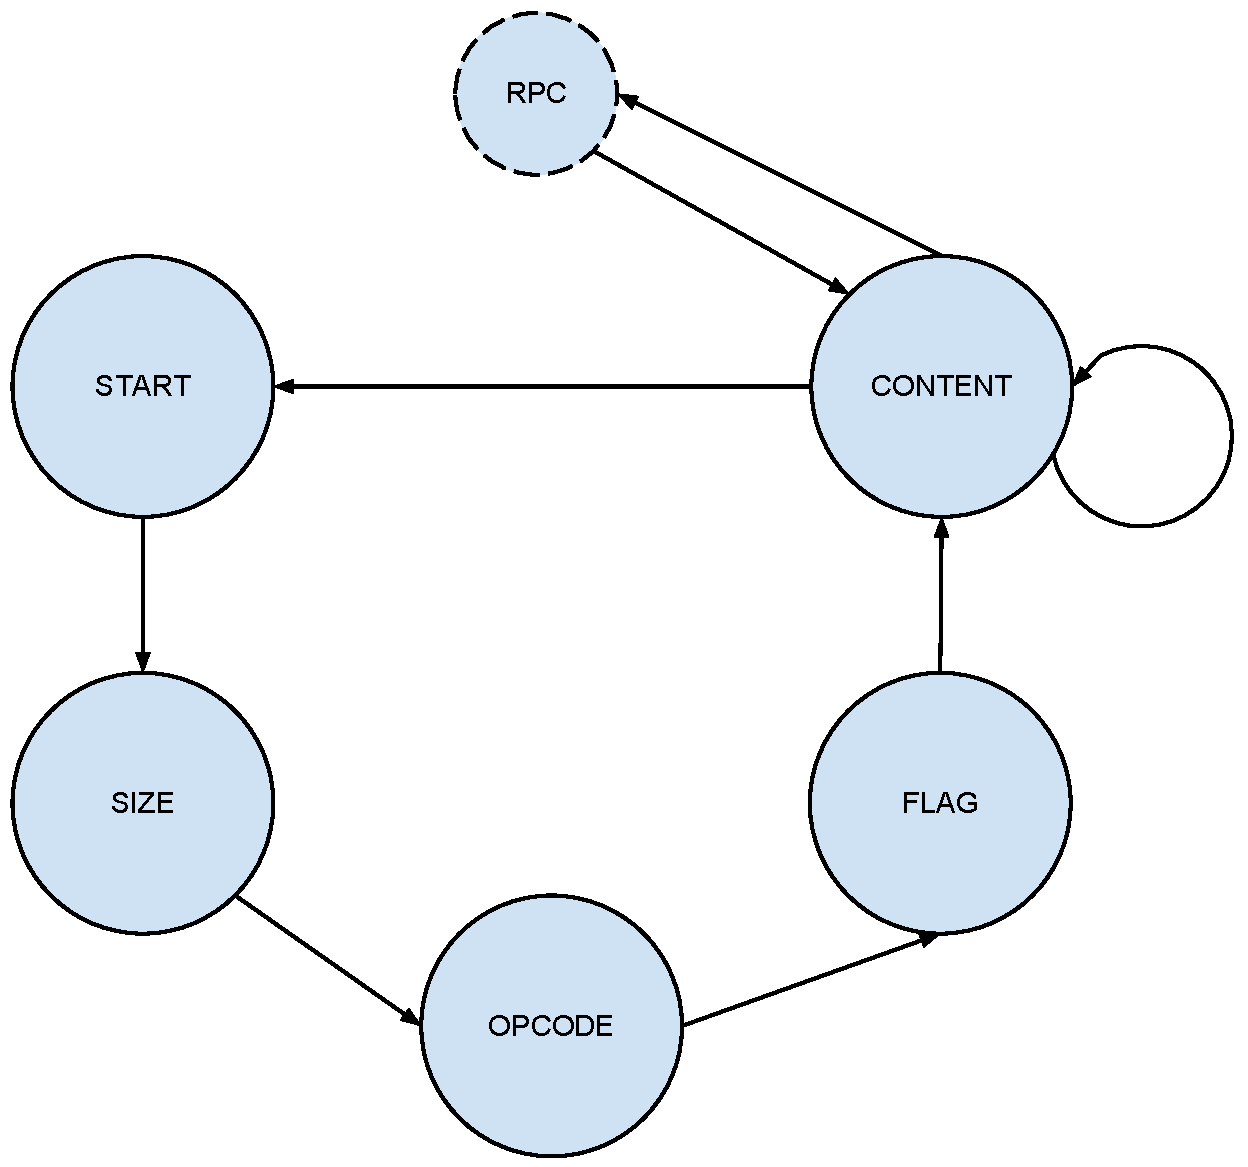
\includegraphics[width=\textwidth, keepaspectratio]{img/arduino_state-machine.pdf}
\caption{The Arduino state-machine}
\label{fig:arduino_states}
\end{figure}

\begin{table}
\begin{tabular}{c|c|c|c|c|c|}
\cline{2-6}
& \textbf{Start-byte} & \textbf{Size} & \textbf{Opcode} & \textbf{Flag} & \textbf{Content} \\
\hline
\multicolumn{1}{|c|}{\textbf{Size}} & 1 & 1 & 1 & 1 & 1-252 \\
\hline
\end{tabular}
\caption{Byte-structure of instructions}
\label{tbl:instr_struct}
\end{table}

\newpage
\section{Applications and Services}

\subsection{T-Shirt application}

As discussed in chapter 5.2 the T-Shirt application design had to be reviewed after roughly one month.

\begin{figure}[h!]
\centering 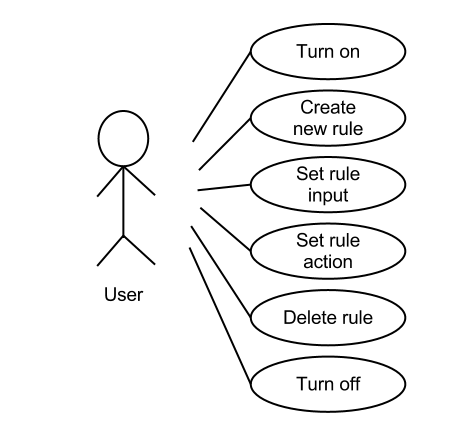
\includegraphics[scale=0.35]{img/design-tshirtappusecase2}
\caption{Use case for the T-Shirt application}
\label{fig:design-tshirtappusecase2}
\end{figure}

For completeness we present the previous application use case in figure \ref{fig:design-tshirtappusecase1}

\begin{figure}[h!]
\centering 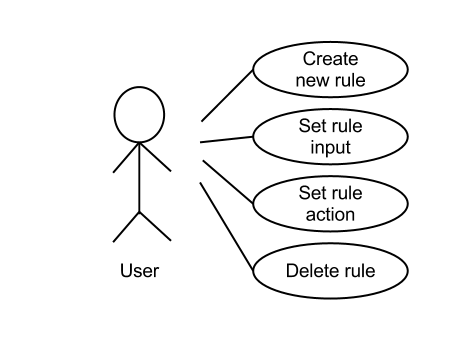
\includegraphics[scale=0.35]{img/design-tshirtappusecase1}
\caption{Initial use case for the T-Shirt application}
\label{fig:design-tshirtappusecase1}
\end{figure}

\subsection{Facebook application}

As discussed in chapter 5.2 the Facebook application design had to be reviewed after roughly one month.

\begin{figure}[h!]
\centering 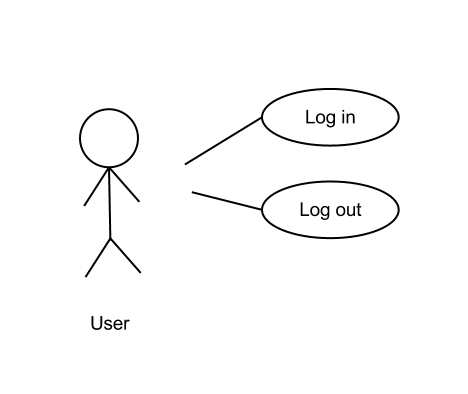
\includegraphics[scale=0.35]{img/design-socialappusecase2}
\caption{Use case for the Social application}
\label{fig:design-socialappusecase2}
\end{figure}

For completeness we present the previous application use case in figure \ref{fig:design-socialappusecase1}.

\begin{figure}[h!]
\centering 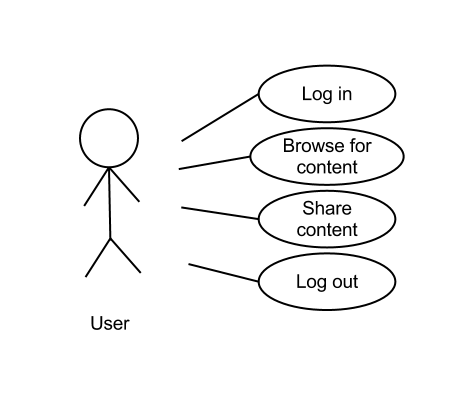
\includegraphics[scale=0.35]{img/design-socialappusecase1}
\caption{Initial use case for the Social application}
\label{fig:design-socialappusecase1}
\end{figure}


\newpage
\section{Prototypes}
Three different prototypes will be produced for the project. They serve both as a proof of concept and
to test that the library works. Each of the prototypes should be different to show that the library can be
used to quickly prototype Arduino Tangible User Interfaces. One of the protoypes, the T-Shirt, is significantly
bigger and more complex than the other two. The T-Shirt is the main prototype of the project; the purpose of the other two
is just to show that the libraries can be use for other applications and in different contexts.

\subsection{The social T-Shirt}
	
\begin{wrapfigure}{r}{0.5\textwidth}
\vspace{-20pt}
\begin{center}
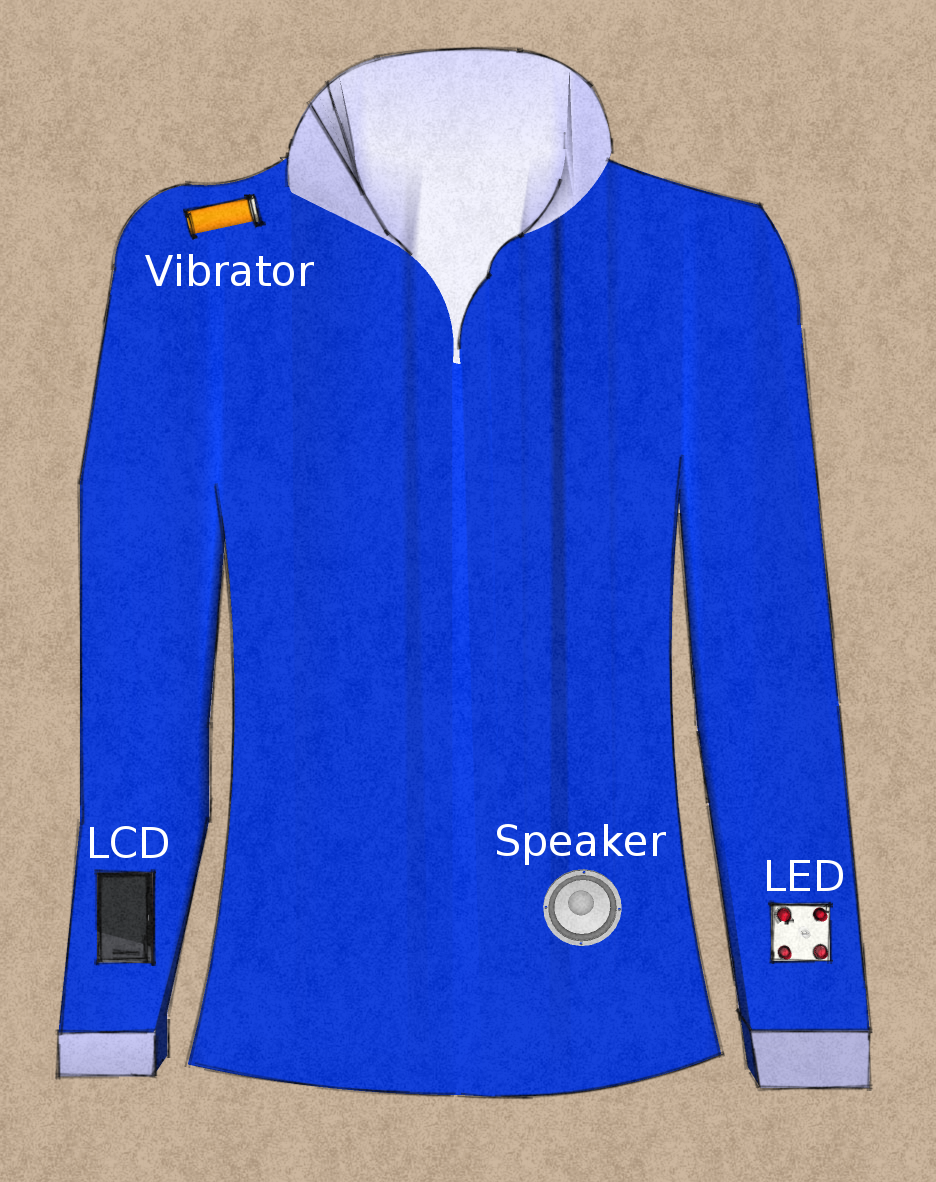
\includegraphics[scale=0.2]{img/design-tshirtproto}
\end{center}
\vspace{-10pt}
\caption{Concept drawing of the T-Shirt Prototype}
\label{fig:design-TShirt}
\vspace{-50pt}
\end{wrapfigure}
	
This is our main prototype and will showcase a lot features.
It consists of a T-Shirt or sweater connected to a Lilypad Arduino that will feature
several displays and indicators which will receive social data from the Android phone.
The shirt features different tangible interfaces (see figure \ref{fig:design-TShirt}):
	
\begin{itemize}
\item LEDs
\item LCD Display
\item Sound speaker
\item Vibration module
\end{itemize}
	
Any of these can be mapped to a fair deal of concepts found in social network.
So a "Poke" from Facebook could become a vibration on the T-Shirt. When someone "Likes" your post a small sound effect
could be played, a LED blinking on status updates from Twitter, etc. The T-Shirt is connected to the social networks
throu a wireless connection to the Android mobile. Specifically, the mobile Android is connected to the internet
and carried in the pocket of the person using the T-Shirt and is connected wirelessly with the Arduino Lilypad through Bluetooth.
	
	%\begin{figure}[h!]
	%\centering 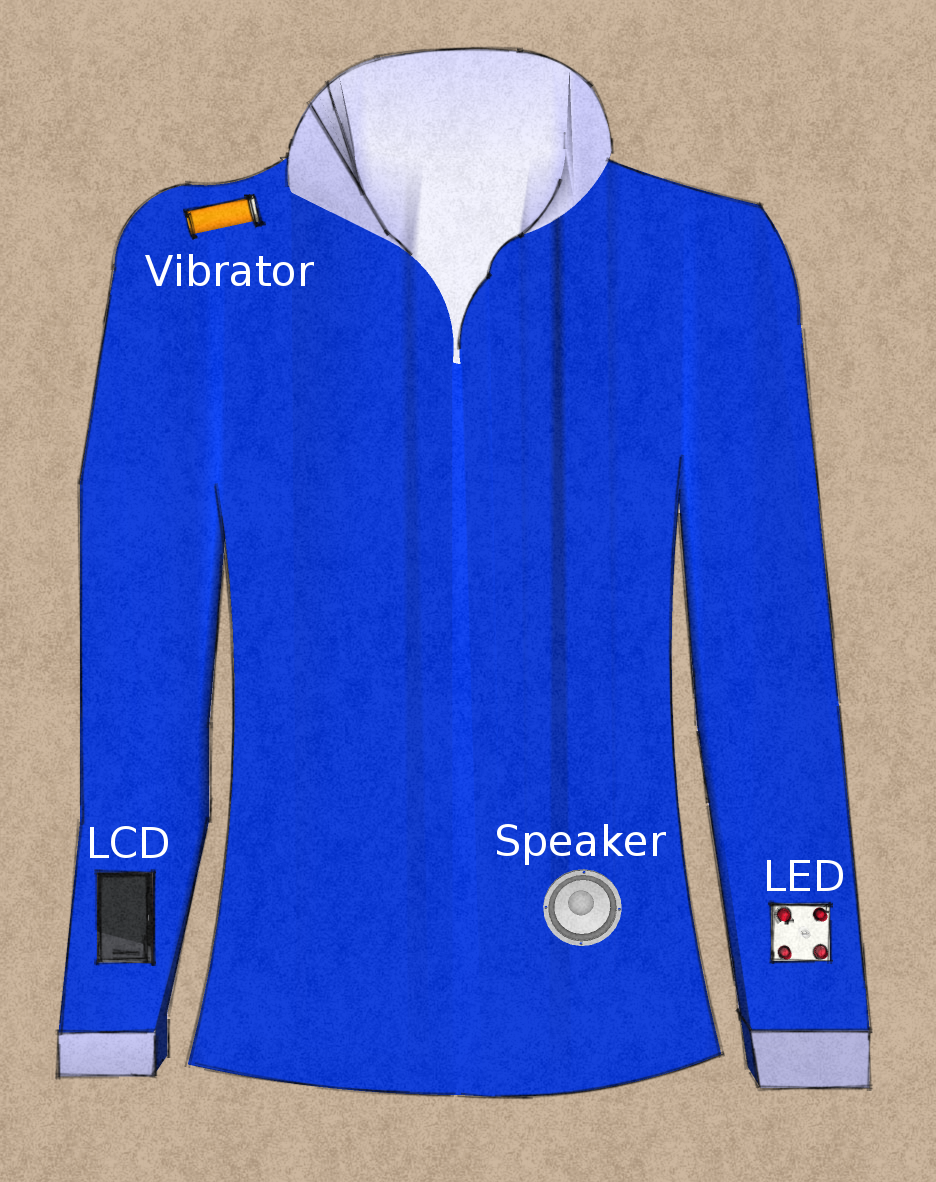
\includegraphics[width=1.0\textwidth]{img/testing-tshirtproto}
	%\caption{Concept drawing of the T-Shirt Prototype}
	%\label{fig:testing-TShirt}
	%\end{figure}

\newpage
	
\subsection{Prototype 2: Temperature Sensor for Android}
This prototype will primarily showcase the communication from Arduino to Android using our libraries.
A temperature sensor will be connected to an Arduino board and then constantly send its output over bluetooth to a
an Android application.
	
\subsection{Prototype 3: Wearable Pictures}
This prototype was first planned to be LED lights showing what mood you had on MySpace. Red LED lights would be angry,
green would be happy and so on. We discovered that MySpace had removed this feature from their pages, even if it was
still supported by the API. It would be a fools errand to pursue something you could not test properly
in a real world situation, so we changed the concept of this prototype. It ended up to be a sort of wearable fashion.
The user can take a picture or choose one on his Android mobile and send it to the prototype Android application.
The picture is then sent with an Intent using the Android API, making it easy to start our program and receive
the bundled picture. For prototyping purposes the wearable product will feature just a few LEDs which our Android
prototype program will map to certain pixels and then transmit over Bluetooth to the Arduino
component and this will promptly light the LEDs.


\newpage

\section{Architecture diagram}
\todo{
	review and remove: expanded and wrote somewhere else.
}
The API layer is the social service layer. It uses androids built in Intents and Messenger class to communicate between social
services and applications. Using these two classes we send JSONObject strings including data wrapped as social concepts such as Person, Group,
Stream, Message, Activity etc. Multiple apps can use the API layer to send and retrieve this data.

Example:
The API layer is connected with twitter. Twitter retrieves a new post and the API layer sends out
a broadcast intent telling a new Message has arrived. The android OS see who are listening to this type of intent and relay
the message to all connected apps. The Developed app will now connect to the Twitter service to fetch the Message.

The bluetooth protocol in the application is a framework that the developed application includes
to be able to send and recive raw data from the arduino board. It includes handshake and
confirmation commands that is similar to tcp.

The arduino board includes a wrapper around the input/output of the firmware to connect to our protocol.

\section{Package Structure}
The system can be divided into smaller sections. This section describes some of the structures
we have divided the system into. The most obvious distinction is between the Java code runs
on the Android platform and the C code which is executed by the Arduino platform.
The Java code is again divided into packaged libraries as described below.

\subsection{Java Code}
\begin{itemize}
\item{no.ntnu.osnap.com}\newline
Communication Library contains every class to establish a connection with a remote device using a general protocol interface. The actual details of the communication such as
Bluetooth, cable, WiFi, stream-based or sockets are hidden away from the user. This is to provide a simple and generic interface to all supported communication methods. The
user can easily add new communication types by extending an abstract class.pdf
\item{no.ntnu.osnap.com.testing}\newline
Test units and sample programs for the ComLib. These are simple test applications that are run on the Android to test if the ComLib is communication correctly using the specified
protocol.
\item{no.ntnu.osnap.social}\newline
Social Library provides an easy to use interface between social networks such as Facebook, Twitter and Myspace and any application or service running on the Android platform.
The SocialLib also provides some general data models such as Person, Group or Post which are concepts that are similar between any social network. 
\item{no.ntnu.osnap.social.testing}  \newline
Test units and sample programs for the SocialLib.
\end{itemize}

\subsection{Arduino C code}
C source code for the Arduino firmware supporting the ComLib protocol.


\section{Use cases}
\todo{
	review.
}
Use Case:
We have two actors we are working with. One is the developer creating the application using our framework.
The other one is the end user with the final product. We are not directly working with the end user as an actor,
but we still want to make our framework so it is simple for developer to have a product with an easy connection to the arduino board.

Our focus on the actor developer is centered around the software he create. We do not know, and we don't need to
know what product he is making. We will work on two parts he can to implement in his software. It will be the setup and
transfer protocol to arduino and Intents to send and recive updates from social services.

For the end user, we want the setup to connect his phone to the developer to be as easy as possible. The focus will be on
simplified connection to arduino board, and easy connection to social services from application.

\todo{
	outdated?
}
\begin{figure}[hb!]
\centering 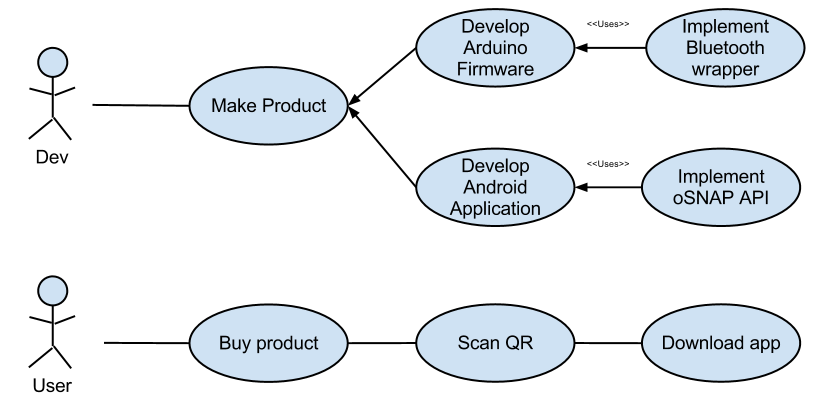
\includegraphics[scale=0.50]{img/use-cases.png}
\caption{Use cases}
\label{fig:architecture-usecases}
\end{figure}
